\documentclass[11pt,a4paper]{scrartcl}

% ********************************************************************    
% Packages
% ********************************************************************
\usepackage[utf8]{inputenc}
\usepackage{tikz}
\usetikzlibrary{shadings}
\usepackage[outline]{contour}
\usepackage{pgfplots}
% \usepackage{tikz-3dplot}
\usepackage{graphicx}
\usepackage{algorithm}% http://ctan.org/pkg/algorithms
\usepackage{algpseudocode}% http://ctan.org/pkg/algorithmicx
\usepackage{subfig}
\usepackage{amsmath,amssymb}
\usepackage{mathtools}
\usepackage{braket}
\usepackage{hyperref}
\usepackage{slashed}
\usepackage{pifont}
\usepackage{tcolorbox}
\usepackage{qcircuit}
\usepackage{amsthm}
\usepackage{amsfonts}
\usepackage{lmodern}
\usepackage{dsfont}
\usepackage{times}
\usepackage{bbm}
\usepackage{wrapfig}
\usepackage[T1]{fontenc}

\usepackage[backend=bibtex,citestyle=authoryear,isbn=false,url=false,doi=false]{biblatex}
\addbibresource{Bibliography.bib}

\DeclareMathOperator{\Tr}{Tr}
\newcommand{\R}{\mathbb{R}}
\newcommand{\N}{\mathbb{N}}
\newcommand{\C}{\mathbb{C}}
\newcommand{\Z}{\mathbb{Z}}

\newtheorem{lemm}{Lemma}

% ********************************************************************    
% Settings
% ********************************************************************

% biblatex
\DeclareCiteCommand{\myfootcite}
  {\footnotetext{\usebibmacro{prenote}}
  {\usebibmacro{citeindex}%
    \usebibmacro{author}
    \printfield{journaltitle}
    \printfield{volume}
    (\printfield{year})}
  {\multicitedelim}
  {\usebibmacro{postnote}}}



%TODO Name does not appear, layout
% meta
\author{Daniel Brosch}
\title{Quantum SDP-solver}
\date{
  Convex Optimization Seminar \\
  Bad Honnef \\
  August 7 -- 9, 2017
}

\begin{document}
\maketitle
{
\centering
\Large
\vspace{4cm}
Mathematisches Institut\\
Mathematisch-Naturwissenschaftliche Fakultät\\
Universität zu Köln\\
}

\thispagestyle{empty}
\newpage
\pagenumbering{roman}
\tableofcontents
\thispagestyle{empty}
\newpage
\pagestyle{headings}
\pagenumbering{arabic}

\section{Introduction}
\subsection{Quantum computing}
%TODO quantum registers, tensor product, matrix register multiplikation
TODO
\subsection{Semidefinite programming}
Semidefinite programming can be used to solve a wide range of problems, some examples include solving graph problems (e.g. approximating MAXCUT), machine learning (e.g. face recognition) and general polynomial optimization. This means that faster SDP-solvers would have potential uses in many different fields, and a fast quantum-SDP-solver could open ways to multiple new applications for quantum computers.
The general form of a semidefinite program is:
\begin{align*}
\text{Primal form:}\quad && \text{Dual form:}\quad &\\
\sup\quad &\Tr(CX) &\inf\quad &b^T y\\
\text{s.t.}\quad &\Tr(A_jX)\leq b_j \text{ for }1\leq j\leq m &\text{s.t.}\quad &\sum_{j=1}^m y_j A_j-C\succeq 0\\
& x\succeq 0 && y\geq 0
\end{align*}
%TODO which norm is this exactly?
Where $A_1,\ldots, A_m, C$ are hermitian matrices. During this work we will assume that $\|A_j\|\leq 1$ and $\|C\|\leq 1$, which is not a restriction, because we can scale $A$, $C$ and $b$ equally without changing the problem (We just have to remember to scale the supremum/infinum back at the end). But we will further assume that we know positive constants $R$ and $r$, so that there is an optimal solution of the primal problem with $\Tr X\leq R$ ($A_1=\mathbbm{1}$, $b_1=R$) and similarily an optimal solution of the dual problem with $\|y\|_1\leq r$. 

\subsection{Arora-Kale SDP solver}
%TODO
The quantum algorithm, which is this paper about, is based on a classical algorithm developed by Arora and Kale. It is an SDP-solver in the form of a matrix multiplicative weight algorithm. While I wont go into details of its workings here (for that I refer to Markus' part of the presentation or (TODO arora kale source)), we need to understand some parts: The basic idea of the algorithm is to start with a positive semidefinite canditate solution $X^{(1)}$ (which does not have to be a feasible solution), then use it with a subroutine called Oracle to find a candidate  dual solution (again not necessarily feasible) $y^{(1)}$, with $b^Ty\leq\alpha$. The value $\alpha$ is here a guess for the optimal value of the SDP, for which we can do a binary search by repeating the algorithm. With this $y$ we can then find a better candidate for the primal solution and repeat this whole process. It can be shown that after enough repetitions the average of all the $y^{(i)}$ is close to dual feasible, and can be tweaked to get a dual feasible solution with $b^Ty\leq\alpha$.

The quantum speed-ups both have to do with the Oracle, so we will take a closer look at it here. Its task is to find a candidate dual solution $y$ from the polytope

\begin{align*}
\mathcal{P}_\varepsilon (X^{(i)})=\{y\in\R^m | &b^Ty\leq\alpha,\\
 &\Tr\left(\left(\sum_{j=1}^m y_jA_j-C\right)X^{(i)}\right)\geq -\varepsilon,\\
 & y\geq 0\}
\end{align*}

The second line is a relaxation of the constraint of the dual programm, which required that $\sum_{j=1}^m y_jA_j-C$ is positive semidefinite.  Instead it only requires the inner product with a specific positive semidefinite matrix not to be too negative. 
Now we can see that we dont even need to know every entry of the matrices $A_j, C$ and $X^{(i)}$, instead it is enough to know the trace inner products between them:

\begin{equation*}
\Tr\left(\left(\sum_{j=1}^m y_jA_j-C\right)X^{(i)}\right)=\sum_{j=1}^m y_j \Tr(A_jX^{(i)})-\Tr(CX^{(i)})
\end{equation*}

It will be easier to work with normalized $\rho=\frac{X^{(i)}}{\Tr(X^{(i)})}$ instead of $X^{(i)}$, and it does not change this polytope if we scale $\varepsilon$ accordingly (remember: we know an upper bound $\Tr(X)\leq R$). And we can further see that additive approximations to these are enough as well: If we have $|a_j-\Tr(A_j\rho)|\leq \theta$ and $|c-\Tr(C\rho)|\leq \theta$ and include the upper bound for an optimal solution $\|y\|_1\leq r$ we can define a new polytope:

\begin{align*}
\tilde{\mathcal{P}}(a_1,\ldots, a_m,c)=\{y\in\R^m | &b^Ty\leq\alpha,\\
&\|y\|_1\leq r,\\
 &\sum_{j=1}^m y_j a_j\geq c,\\
 & y\geq 0\}
\end{align*}

Notice here that $\varepsilon$ does not appear in this formulation. This is because we can show that if we have a $y\in\mathcal{P}_0(X)$ with $\|y\|_1\leq r$, then

\begin{equation*}
0\leq \sum_{j=1}^m y_j \Tr(A_j\rho)-\Tr(C\rho) \leq \sum_{j=1}^m y_j (a_j+\theta)-(c-\theta) \leq  \sum_{j=1}^m y_j a_j-c +(r+1)\theta
\end{equation*}

which shows that $y$ is in $\tilde{\mathcal{P}}(a_1,\ldots,a_m, c'=c-(r+1)\theta)$. This means, because when there is a feasible solution, then $\mathcal{P}_0(\rho)$ is not empty, that $\tilde{\mathcal{P}}(a_1,\ldots,a_m, c')$ is not empty as well. It does work other way around as well: If we have a $y\in\tilde{\mathcal{P}}(a_1,\ldots,a_m, c')$, then is $y\in \mathcal{P}_{4Rr\theta}(X)$.

This means that we can work with $\tilde{\mathcal{P}}$ instead of $\mathcal{P}$ in the algorithm. Both of the quantum speed-ups have to do with this oracle.

% ************************************
\section{Quantum Speed-Ups}
% ************************************

The algorithm of Arora and Kale can be sped up using quantum computers at two points, the first of which is estimating $\Tr(A\rho)$ for a hermitian matrix $A$ and a density matrix $\rho = \frac{e^{-H}}{\Tr(e^{-H})}$, which is used as input for the Oracle.

The second speed-up is the implementation of the (general) oracle itself, which will be based on applications of known quantum algorithms.

\subsection{The input of the Oracle:}

For the oracle's input we have to approximate expressions of the form $\Tr(Ap)$ with $p=\frac{e^{-H}}{\Tr(e^{-H})}$, where $A$ is a hermitian matrix, and $H$ is positive semidefinite. This we can seperate into two calculations, $\Tr(Ae^{-H})$ and $\Tr(e^{-H})$.

Important to note is here that we wont calculate these values in binary directly, instead it will first be the probability of a qubit being 0 (amplitude of the qubit). Specifically this means we have to construct a quantum circuit, which corresponds to a unitary matrix $U$, in a way so that it turns a specific input register (e.g. $\ket{0\ldots 0}$) into a register with the first qubit as wanted.

Amplitude estimation is then used to approximate this probability, during which $U$ and $U^{-1}$ are used multiple times. The amount of uses depends inversely on a lower bound of this probability, which we can increase by altering the input slightly without changing the output.

\vspace{1cm}

Before explaining how to construct this circuit (or at least its general idea) for any semidefinite programm, we will take a look at the much simpler case of \textbf{linear programming}. These can be seen as the subclass of SDP, which only uses diagonal matrices. Here it means that the calculation of $\Tr(Ae^{-H})$ becomes significantly easier (and by that the one of $\Tr(e^{-H})=\Tr(\mathbbm{1}e^{-H})$ as well), as it is now just the sum of $A_{ii}e^{-H_{ii}}$ for $1\leq i\leq n$.

If we were to approximate this classically, we would have to calculate these $n$ values seperately, which would give us a runtime of at least $\mathcal{O}(n)$. Even just reading the input values would give us this runtime already classically. But if we use a quantum circuit, we will only need a single call to the input circuits for $A$ and $H$, and a single call to a circuit which calculates $ae^{-h}$. To do this we will start with an all-zero register of $\log(n)$ qubits, which is enough for a binary representation of $i$:

\begin{equation*}
\ket{0\ldots 0}
\end{equation*}

Now we are going to do something that can not be done classically: We will turn this register into an equal superposition of all the $i$ from $1$ to $n$. This means that if we were to measure all qubits, we would measure each $i$ with equal probability. Every qubit will have a $50\%$ chance to be $0$ or $1$, independently from another, which means that this state is not entangled. To construct this state we will apply a so called hadamard gate to each of the $log(n)$ qubits, which turns $\ket{0}$ into $\frac{1}{\sqrt 2}(\ket{0}+\ket{1})$:

\begin{equation*}
\frac{1}{\sqrt{n}}\sum_{i=1}^n\ket{i}
\end{equation*}

At this point we have to take a look at how we access the diagonal matrices $A$ and $H$. We cannot use a circuit which would turn $\ket{i}$ into $\ket{A_{ii}}$, because in general this is not a reversible operation. But what can be done is to use a circuit which sends $\ket{i}\ket{z}$ to $\ket{i}\ket{z\oplus A_{ii}}$, and a circuit which sends it to $\ket{i}\ket{z\oplus H_{ii}}$. These circuits we will call $O_A$ and $O_H$. The operator $\oplus$ is a bitwise exclusive-or operation, which means that $\ket{0\oplus A_{ii}}=\ket{A_{ii}}$. If we now add enough zero-initialised qubits to the end of the register to store one entry of $A$ and $H$, we can apply these two circuits to them and the qubits we had before. This kind of qubits we call "ancilla qubits", which will be used in most of the steps of this circuit. This leaves us with the register:

\begin{equation*}
\frac{1}{\sqrt{n}}\sum_{i=1}^n\ket{i}\ket{H_{ii}}\ket{A_{ii}}
\end{equation*}

To do this we only had to apply $O_A$ and $O_H$ once. Notice here that those values are "stored" in the same qubits, which means that we could not use this to read out all the values $H_{ii}$ and $A_{ii}$ seperately. But we could, if we wanted to, measure the first few qubits to get a random $i$, which would tell us that the state "collapsed" to $\ket{i}\ket{H_{ii}}\ket{A_{ii}}$. We could then measure the remaining bits to get $H_{ii}$ and $A_{ii}$. Another interesting thing about this state is that it is an entangled state, except if $A_{ii}=A_{11}$ and $H_{ii}=H_{11}$ for all $i$. An example would be $n=2$, $A_{ii}=H_{ii}=i$, in which case the state would be $\frac{1}{\sqrt{2}}(\ket{000}+\ket{111})$. Its qubits are not independent, because the three qubits always have the same state, even if the first one measured is random.

So at this point we have read all the input values we need, while only needing the time it would take to read one of them classically. Next we are going to calculate the values $A_{ii}e^{-H_{ii}}$, first as binary values using multiple qubits. Similar to before we cannot calculate these values "in-place", but instead use more ancilla qubits and a circuit $\ket{h}\ket{a}\ket{z}\to\ket{h}\ket{a}\ket{z\oplus f(h,a)}$. We could now set $f(h,a)=ae^{-h}$, but to be able to sum them efficiently later we need to do turn these binary values first into "amplitudes" of qubits, their probability to be measured as $\ket{0}$.

Lets say we have a value $b\in [0,1]$, stored as a binary value in multiple qubits, which we want to turn into the probability of a qubit being 0. To do this we have to calculate an approximation of $\arcsin(\sqrt{b})/\pi\approx \beta=b_0.b_1b_2b_3\ldots b_t$. Using one ancilla qubit we are now working with the register $\ket{1}\ket{\beta}=\ket{1}\ket{b_0}\ket{b_1}\ldots\ket{b_t}$. If we now apply $t$ "controlled" rotations to the first qubit, one for each bit of $\beta$, rotating by $\pi 2^{-j}$ towards $\ket{0}$ if $b_j=1$, we receive:
\begin{align*}
&\left(\sin\left(\sum_{b_i=1} \pi 2^{-i}\right)\ket{0}
+\cos\left(\sum_{b_i=1} \pi 2^{-i}\right)\ket{1}\right)
 \ket{\beta}\\
=&\left(\sin\left(\pi\beta\right)\ket{0}
+\cos\left(\pi\beta\right)\ket{1}\right)
 \ket{\beta}\\
=&(\sqrt{b}\ket{0}+\sqrt{1-b}\ket{1})\ket{\beta}
\end{align*}
For which the probability, that the first qubit is 0, is exactly $\|\sqrt{b}\ket{0}\|^2=b$.

To be able to use this transformation on our register, which is still in the state $\frac{1}{\sqrt{n}}\sum_{i=1}^n\ket{i}\ket{H_{ii}}\ket{A_{ii}}$, we have to approximate $\arcsin(\sqrt{b_i})/\pi$ for $b_i=A_{ii}e^{-H_{ii}}$. Note here that the $b_i$ are not necessarily in $[0,1]$ in this form. This can fixed by shifting and scaling $A$, but let us here just assume that the $b_i$ are values in $[0,1]$. We could now find a classical circuit only using logic gates which calculates $f(h,a)\approx \arcsin(\sqrt{ae^{-h}})/\pi$, which we can then turn into a quantum circuit using reversible gates. As explained before this circuit has to be of the form $\ket{h}\ket{a}\ket{z}\to\ket{h}\ket{a}\ket{z\oplus f(h,a)}$. Applying this to our register (using new ancilla qubits initialised with zero at the end) turns it into:

\begin{equation*}
\frac{1}{\sqrt{n}}\sum_{i=1}^n\ket{i}\ket{H_{ii}}\ket{A_{ii}}\ket{\beta_i}
\end{equation*}

To this we add another ancilla qubit (this time initialised as 1) at the beginning, on which we then use the circuit which calculates $\ket{1}\ket{\beta}\to (\sin(\pi\beta)\ket{0}+\cos(\pi\beta)\ket{1})\ket{\beta}$ from above:

\begin{equation*}
\frac{1}{\sqrt{n}}\sum_{i=1}^n\left(\sqrt{A_{ii}e^{-H_{ii}}}\ket{0}+\sqrt{1-A_{ii}e^{-H_{ii}}}\ket{1}\right)\ket{i}\ket{H_{ii}}\ket{A_{ii}}\ket{\beta_i}
\end{equation*}

The 2-norm of the parts of this register where the first qubit is zero is its probability to be measured as zero. This is here:

\begin{equation*}
\left\|\frac{1}{\sqrt{n}}\sum_{i=1}^n\sqrt{A_{ii}e^{-H_{ii}}}\ket{i}\right\|^2=\frac{1}{n}\sum_{i=1}^n A_{ii}e^{-H_{ii}}=\frac{1}{n}\Tr(Ae^{-H})
\end{equation*}

That means we have now constructed the circuit we wanted, which uses $log(n)$ Hadamard-gates, two input gates, a single arithmetic circuit, and $\mathcal{O}(\log(1/\varepsilon))$ rotation gates. %TODO Check this

%TODO draw circuit? 
%\Qcircuit @C=1em @R=1em {
%      \lstick{\ket{q_1}} & \gate{U_1} & \qw & \multigate{1}{U_3} & \meter  \\
%      \lstick{\ket{q_2}} & \qw & \multigate{1}{U_2} & \ghost{U_3} & \meter \\
%      \lstick{\ket{q_3}} & \qw & \ghost{U_2} & \qw & \meter
%    }

\vspace{1cm}

The general \textbf{semidefinite programming} case is much more complicated. Here is $A$ a hermitian matrix with $\|A\|\leq 1$, $H$ is a positive semidefinite matrix, and we have to calculate $\Tr(Ae^{-H})$. Essentially we are going to need circuits which apply the matrices $\sqrt{A}$ and $\sqrt{e^{-H}}=e^{-H/2}$ to their input register. The roots come from us taking the 2-norm of the register later to calculate the probability of some qubits being zero.

But there is a problem: Those matrices are not unitary, which means that we cant implement them as quantum circuits directly, as those have to be unitary (and by that reversible). But what we do know is that they are "norm-decreasing", their operator norms are smaller or equal to 1. This means that we can "add" something to them to make them unitary. This can be done in a way which allows us to seperate the original operation and the part that was added:

\begin{equation*}
U_B\ket{0}\ket{\psi}=\ket{0}B\ket{\psi}+\ket{1}*
\end{equation*}

This means that the circuit $U_B$ applies the Operation $B$ (here $\sqrt{A}$ or $e^{-H/2}$) to the vector $\ket{\psi}$, if we measure the new ancilla qubit as $0$. Remember here that we identify the hilbert space of the $log(n)$ qubits with $\C^n$, $\ket{i} \hat{=} e_i$, for the matrix multiplication. This means that this operation could turn the basis-states $\ket{i}$ into an entangled superposition of multiple states. We can apply both matrices to the same vector by using a different ancilla qubit for each of the operations:

\begin{align*}
U_{\sqrt{A}}&U_{e^{-H/2}}\ket{0}\ket{0}\ket{\psi}\\
&=U_{\sqrt{A}}(\ket{0}\ket{0}e^{-H/2}\ket{\psi}+\ket{0}\ket{1}*)\\
&=\ket{0}\ket{0}\sqrt{A}e^{-H/2}\ket{\psi}+\ket{0}\ket{1}*+\ket{1}\ket{0}*+\ket{1}\ket{1}*
\end{align*}

Here we can see that both matrices are applied to the input vector if both ancilla qubits are zero. Now we still have to calculate the trace of this matrix. The trace of a matrix $B$ is exactly the sum over $e_i^T Be_i$, which means that we want to somehow apply all the $\ket{i}$ at the same time. This time we cannot just use the superposition of all basis-states $\frac{1}{\sqrt n}\sum_{i=1}^n \ket{i}$, because this would instead apply a scaled all-one vector to the matrices. But we can "seperate" these by using entanglement with another $log(n)$ qubits, and then only applying the matrices to first half. If we set $\ket{\psi}=\frac{1}{\sqrt n}\sum_{i=1}^n \ket{i}\ket{i}$, the probability that the two ancilla qubits are zero after applying both matrices becomes:

\begin{align*}
\left\|\frac{1}{\sqrt n}\sum_{i=1}^n\left(\sqrt{A}e^{-H/2}\ket{i}\right)\ket{i}\right\|^2
&=\frac{1}{n}\sum_{i=1}^n \left(\sqrt{A}e^{-H/2}\ket{i}\right)^\dagger\sqrt{A}e^{-H/2}\ket{i}\\
&=\frac{1}{n}\sum_{i=1}^n \bra{i}\left(e^{-H/2}\right)^\dagger\sqrt{A}^\dagger\sqrt{A}e^{-H/2}\ket{i}\\
&=\frac{1}{n}\Tr\left(\sqrt{A}\sqrt{A}e^{-H/2}e^{-H/2}\right)\\
&=\frac{1}{n}\Tr\left(Ae^{-H}\right)
\end{align*}

We used here that $\sqrt{A}$ and $e^{-H/2}$ are self adjoint, because $A$ and $H$ are self-adjoint. At this point we have nearly constructed the circuit we want, just with the probability of two qubits being zero instead of one. But we could now add another ancilla qubit and use a three-qubit gate, which calculates the logical-and of those qubits and stores the result in the new one, if we wanted to.

Now we still have to construct the circuits $U_{\sqrt{A}}$ and $U_{e^{-H/2}}$. Doing this is a complicated task, but we can take a look at its basic idea. The functions $\sqrt{A}$ and $e^A$ are "smooth functions of hamiltonians", which means that they only change the eigenvalues of hermitian matrices:

\begin{equation*}
f(H)=f(U \mathrm{Diag}(\lambda_1,\ldots, \lambda_n) U^\dagger)=U \mathrm{Diag}(\tilde{f}(\lambda_1),\ldots,\tilde{f}(\lambda_n))U^\dagger
\end{equation*}

And the function $\tilde{f}$ is "smooth" enough on an interval to be approximated using a polynomial. This can then be used to find a fourier series (sum of complex exponentials) approximating the polynomial. The same fourier series can be used to approximate $f$ itself ($e^{iUDU^\dagger}=Ue^{iD}U^\dagger$), and can be implemented efficiently using a quantum computer.



\subsection{The Oracle}

The Oracle is a subroutine used by the Arora-Kale algorithm, which calculates a candidate dual solution $y$ using a candidate primal solution $X$. As seen earlier it is not necessary for the oracle to know each entry of the semidefinite matrix $X$, instead it can use $a_j\approx\Tr(A_j\rho)$ for $j=1,\ldots,m$ and $c=\Tr(C\rho)-\varepsilon$. That means we have to calculate a $y\in \mathbb{R}^m$ with:

\begin{align*}
\|y\|_1&\leq r & \omit\rlap{Compared to the dual SDP:}\\
b^T y&\leq \alpha&\min \quad &b^T y\\
a^T y&\geq c& \text{s.t. } &\sum_{j=1}^m y_j A_j - C\succeq 0\\
y&\geq 0 & &y\geq 0
\end{align*}

The first condition $\|y\|_1\leq r$ is no restriction, because we assumed that there is an optimal solution with this property. We are now going to simplify the problem, starting by substituting $y$ with $Nq$ where $N=\|y\|_1$ and $\|q\|_1=1$. This results in the problem:

%Some ugly magic for rcases inside of align
\begin{equation*}
 \begin{split}
  b^T q&\leq \alpha/N\\
  a^T q&\geq c/N\\
  \begin{aligned}
   \|q\|_1\\
   q
  \end{aligned}
  &
  \begin{rcases*}
   =1\\
   \geq 0
  \end{rcases*} \text{convex combination coefficients}  \\
  0&<N\leq r
 \end{split}
\end{equation*}

This way we recieve a two-dimensional interpretation of the oracle: We want to find the convex combination of a point $P$ in the polytope $Q=\mathrm{conv}\{p_i=(b_i,a_i)\}$, which lies to the upper left of the point $(\alpha/N, c/N)$ for an $N\in (0,r]$. To understand the second condition we define $G_N$ as the upper-left quadrant starting at $(\alpha/N, c/N)$ and $G$ as the union of all the $G_N$ with $0<N\leq r$.

{

\begin{wrapfigure}{l}{0.6\textwidth}
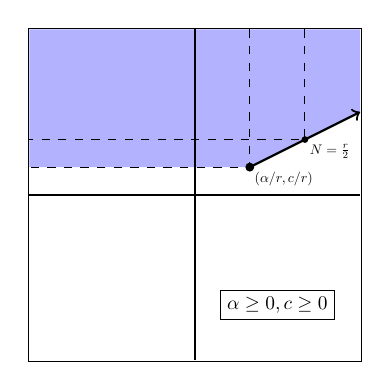
\begin{tikzpicture}[scale=0.7]%[shift={(11cm,-1.5cm)}]
\contourlength{0.5mm};

\coordinate[label={[scale=0.5]below right: {$(\alpha/r,c/r)$}}] (ac) at (1,1/2);
\coordinate[label={[scale=0.5]below right: {$N=\frac{r}{2}$}}]  (ac2) at (2,1);
\coordinate													    (ac3) at (3,3/2);

\fill[blue!30!white] (ac)--(ac -| -3,0)--(-3,3)--(ac3 |- 0,3)--(ac3)--cycle;

\draw[thick] (-3,0)--(3,0);
\draw[thick] (0, -3)--(0,3);
\draw[dashed] (ac |- 0,3) -- (ac) -- (ac -| -3,0);
\draw[dashed] (ac2 |- 0,3) -- (ac2) -- (ac2 -| -3,0);

\filldraw (ac) circle(0.07);
\filldraw (ac2) circle(0.05);

\draw[->, thick] (ac)--(ac3);

\node[scale=0.7,draw] at (1.5,-2) {$\alpha\geq 0, c\geq 0$};
\draw (current bounding box.north east) rectangle (current bounding box.south west);
\end{tikzpicture}
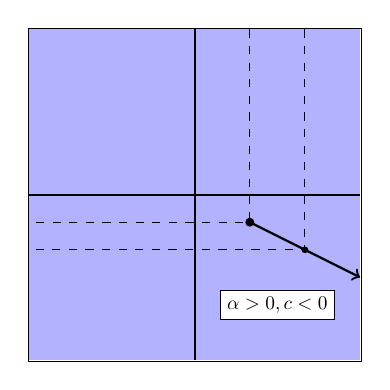
\begin{tikzpicture}[scale=0.7]%[shift={(11cm,-1.5cm)}]
\contourlength{0.5mm};

\coordinate (ac) at (1,-1/2);
\coordinate (ac2) at (2,-1);
\coordinate	(ac3) at (3,-3/2);

\fill[blue!30!white] (-3,-3)--(-3,3)--(3,3)--(3,-3)--cycle;

\draw[thick] (-3,0)--(3,0);
\draw[thick] (0, -3)--(0,3);
\draw[dashed] (ac |- 0,3) -- (ac) -- (ac -| -3,0);
\draw[dashed] (ac2 |- 0,3) -- (ac2) -- (ac2 -| -3,0);

\filldraw (ac) circle(0.07);
\filldraw (ac2) circle(0.05);

\draw[->, thick] (ac)--(ac3);

\node[scale=0.7,draw, fill=white] at (1.5,-2) {$\alpha > 0, c < 0$};
\draw (current bounding box.north east) rectangle (current bounding box.south west);
\end{tikzpicture}

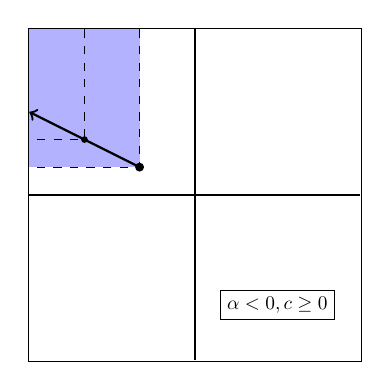
\begin{tikzpicture}[scale=0.7]%[shift={(11cm,-1.5cm)}]
\contourlength{0.5mm};

\coordinate (ac) at (-1,1/2);
\coordinate (ac2) at (-2,1);
\coordinate	(ac3) at (-3,3/2);

\fill[blue!30!white] (ac)--(ac -| -3,0)--(-3,3)--(ac |- 0,3)--cycle;

\draw[thick] (-3,0)--(3,0);
\draw[thick] (0, -3)--(0,3);
\draw[dashed] (ac |- 0,3) -- (ac) -- (ac -| -3,0);
\draw[dashed] (ac2 |- 0,3) -- (ac2) -- (ac2 -| -3,0);

\filldraw (ac) circle(0.07);
\filldraw (ac2) circle(0.05);

\draw[->, thick] (ac)--(ac3);

\node[scale=0.7,draw] at (1.5,-2) {$\alpha < 0, c\geq 0$};
\draw (current bounding box.north east) rectangle (current bounding box.south west);
\end{tikzpicture}
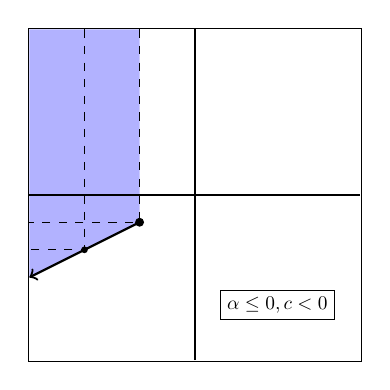
\begin{tikzpicture}[scale=0.7]%[shift={(11cm,-1.5cm)}]
\contourlength{0.5mm};

\coordinate (ac) at (-1,-1/2);
\coordinate (ac2) at (-2,-1);
\coordinate	(ac3) at (-3,-3/2);

\fill[blue!30!white] (ac)--(ac |- -3,3)--(-3,3)--(ac3)--cycle;

\draw[thick] (-3,0)--(3,0);
\draw[thick] (0, -3)--(0,3);
\draw[dashed] (ac |- 0,3) -- (ac) -- (ac -| -3,0);
\draw[dashed] (ac2 |- 0,3) -- (ac2) -- (ac2 -| -3,0);

\filldraw (ac) circle(0.07);
\filldraw (ac2) circle(0.05);

\draw[->, thick] (ac)--(ac3);

\node[scale=0.7,draw] at (1.5,-2) {$\alpha \leq 0, c < 0$};
\draw (current bounding box.north east) rectangle (current bounding box.south west);
\end{tikzpicture}
\end{wrapfigure}

The area $G$ is the union of quadrants which are moved along a ray, starting at $(\alpha/r,c/r)$, in direction $(\alpha,c)$. If the ray is turned towards the bottom right ($\alpha > 0$, $c < 0$), then every point of the whole plane is in a $G_N$. This makes the problem trivial, and we can choose $y=0$ in the original problem. This can be extended to the case $\alpha \geq 0$,  $c \leq 0$, which can be easily checked by setting $y$ to $0$.


Otherwise $G$ is the intersection of two half-planes, at least one of them horizontal or vertical. The corner of this area is always the starting point of the ray.

}

\newpage
\vspace{1cm}

It is easy to see that if there is a solution $q$, then there is also a 2-sparse solution. This means we can always assume that we can find a solution on one of the connecting lines $\overline{p_i p_j}$ of corners of the polytope:

{

\begin{wrapfigure}{r}{6cm}
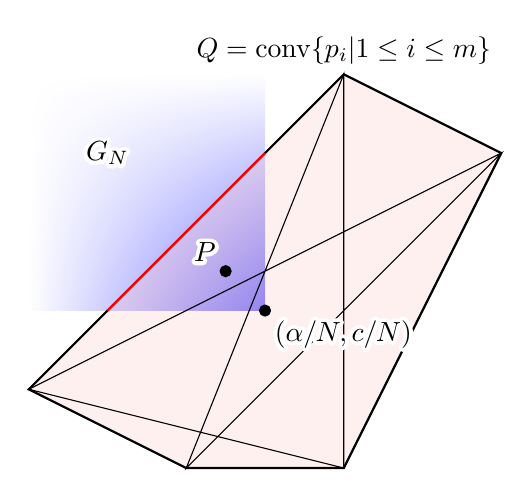
\begin{tikzpicture}
\contourlength{0.5mm};
\shade[lower right=blue!60!white] (0,0) rectangle (3,3);
\node at (1,2) {\contour{white}{$G_N$}};
\filldraw[thick, fill=red!20!white, fill opacity=0.3] (0,-1)--(4,3)--(6,2)--(4,-2)--(2,-2)--cycle;
\draw[red, thick] (1,0)--(3,2);
\node[anchor=south] at (4,3) {$Q=\mathrm{conv}\{p_i|1\leq i \leq m\}$};
\draw (0,-1)--(6,2)--(2,-2)--(4,3)--(4,-2)--cycle;
\filldraw (2.5,0.5) circle(0.07) node[anchor=south east]{\contour{white}{$P$}};
\filldraw (3,0) circle(0.07) node[anchor=north west]{\contour{white}{$(\alpha/N,c/N)$}};
\end{tikzpicture}
\end{wrapfigure}

In the algorithm we will check if there is a $p_i\in G$ seperately, so we will assume that there is no such $p_i$ at this point. But if there is a point $P\in G_N\cap Q$,	then a part of the boundary of the polytope has to cross (or at least touch) $G_N$. This is because $G_N$ is unbounded, so it cant lie inside of $Q$ completely, and $Q$ is a polytope with no corners inside of $G_N$. The boundary of $Q$ is a subset of connecting lines of corners of the polytope, which we can generalize to say that there is a line between corners with $\overline{p_i p_j}\cap G_N\neq\emptyset$.

That means we can always find a 2-sparse solution $q$, because we can describe those lines as convex combinations of its two ends.

}

\vspace{1cm}

At this point we can take a look at the algorithm for the Oracle. It consists of three steps:

\begin{algorithm}
\caption{ORACLE}
\begin{algorithmic}
\If{$\alpha\geq 0$ and $c\leq 0$}
	\Comment{Step 1: Check if $G$ is all of $\R^2$}
    \State \Return $y=0$
\ElsIf{$\exists i: p_i\in G$}
	\Comment{Step 2: Check if one of the corners is in $G$}
    \State \Return $y=Ne_i$ with $N=c/a_i$
\Else
	\Comment{Step 3: Search a 2-sparse solution}
	\State Find $j,k$ such that $\overline{p_j p_k}\cap G\neq \emptyset$
	\If{Such $j,k$ exist}
		\State Calculate a fitting convex combination $q$ and scalar $N$
		\State \Return $y=Nq$
	\Else
		\State \Return	No $y$ found.
	\EndIf
\EndIf
\end{algorithmic}
\end{algorithm}

{

\begin{wrapfigure}{r}{6cm}
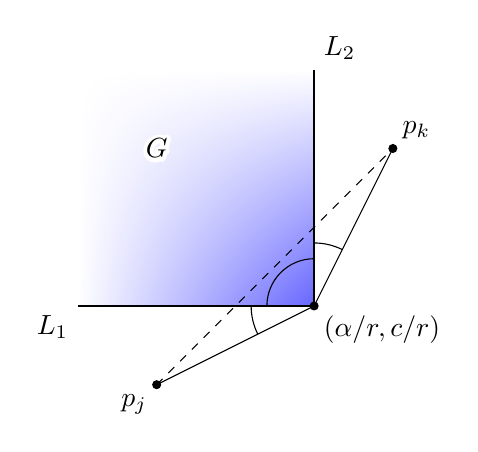
\begin{tikzpicture}
\contourlength{0.5mm};
\coordinate[label=below left:$L_1$] (L1) at (0,0);
\coordinate[label=above right:$L_2$] (L2) at (3,3);
\coordinate[label=below right:{$(\alpha/r,c/r)$}] (g) at (3,0);
\coordinate[label=below left:$p_j$] (pj) at (1,-1);
\coordinate[label=above right:$p_k$] (pk) at (4,2);

\shade[lower right=blue!60!white] (L1) rectangle (3,3);
\draw[thick] (g)--(L1);
\draw[thick] (g)--(L2);
\node at (1,2) {\contour{white}{$G$}};
\filldraw (g) circle(0.05);
\filldraw (pj) circle(0.05);
\filldraw (pk) circle(0.05);
\draw (g)--(pj);
\draw (g)--(pk);
\draw[dashed] (pj)--(pk);

\begin{scope}
\path[clip] (g) -- (pj) -- (L1);
\draw (g) circle (0.8);
\end{scope}
%\node[scale=0.5] at (2.3,-0.1)  {$\sphericalangle p_j L_1$};

\begin{scope}
\path[clip] (g) -- (L1) -- (L2);
\draw (g) circle (0.6);
\end{scope}
%\node[scale=0.5] at (2.6,0.2) {$\sphericalangle L_1 L_2$};

\begin{scope}
\path[clip] (g) -- (L2) -- (pk);
\draw (g) circle (0.8);
\end{scope}
%\node[scale=0.5] at (3.2,0.9) {$\sphericalangle L_2 p_k$};
\end{tikzpicture}
\end{wrapfigure}

Step one and two of the algorithm are straightforward, but how can we find corners with $\overline{p_j p_k}\cap G\neq \emptyset$? We have seen that the area $G$ is the intersection of two half-planes, lets call them $L_1$ and $L_2$. The line $\overline{p_j p_k}$ crosses $G$ if and only if
\begin{equation*}
\sphericalangle p_j L_1+\sphericalangle L_1 L_2+\sphericalangle L_2 p_k\leq \pi
\end{equation*}
	
The angle $\sphericalangle L_1 L_2$ is independent from $j$ and $k$, which means that we can minimize $\sphericalangle p_j L_1$ and $\sphericalangle L_2 p_k$   seperately.

}


\vspace{1cm}

%TODO algo sources
Where is the quantum speed-up? In step two of the algorithm we have to check if one of the $p_i$'s is in $G$. If we implement the function $i\to$"Is $p_i\in G$?" as a  quantum circuit, then Grover search\footnote{The Grover algorithm's idea is to rotate a starting vector to the solution vector. The basic version of the Grover algorithm can only be aplied if there is exactly one solution. It can be shown that if we divide the amount of rotations used by the root of the number of solutions, we can find one of them. In the general case it is enough to do $T$ rotations first and checking the state, then $T/\sqrt 2$, then $T/\sqrt {2^2}$, down to $T/\sqrt {2^{log(m)}}$ [We have to start the process again every time, because measuring states "destroys" them].} can be used to find such a $p_i$ in $\mathcal{O}(\sqrt{m})$. Similarily we have to minimize the angles $\sphericalangle p_j L_1$ and $\sphericalangle L_2 p_k$ for step 3, so if we implement the functions $i\to\sphericalangle p_i L_1$ and $i\to \sphericalangle L_2 p_k$ as quantum circuits, then the quantum minimum-finding algorithm of Dürr and Høyer\footnote{This algorithm works by using the general Grover search repeatedly on "$f(i)\leq t$?", doing an (exponential) binary search for $t$.} can be used to minimize them in $\tilde{\mathcal{O}}(\sqrt{m})$.


%Chapter 4?
\subsection{Runtime of the SDP solver}

The calculation of the runtime is not that complicated, but we would have to use a few formulas we didnt explain or use before. Basically its the number of iterations of the Arora-Kale-Algorithm, multiplied by the amount of uses of values of the form $\Tr(A_j)$ during one oracle call, times the runtime of this value's calculation. The second factor comes from us needing multiple copies of the same values, because quantum computers can only use these once (and cannot create copies). This means we have to calculate them multiple times. As a reminder $m$ is the amount of constraints of the program, $n$ is the size of the matrices, $s$ is the sparsity of the input matrices, $R$ and $r$ are upper bounds on an optimal primal and dual solution, and $\varepsilon$ is the precision of the solutions we want.

For general semidefinite programs we get the runtime:
\begin{equation*}
\tilde{\mathcal{O}}\left(\sqrt{mn}s^2\left(\frac{Rr}{\varepsilon}\right)^8\right)
\end{equation*}
In the linear programming case we get a better runtime. Here we use the LP case of the trace calculation, and all input matrices have sparsity $1$.
\begin{equation*}
\tilde{\mathcal{O}}\left(\sqrt{mn}\left(\frac{Rr}{\varepsilon}\right)^5\right)
\end{equation*}
If we implement all steps of this algorithm classically, we get a worse runtime in $n$ and $m$, but a better one in the remaining parameters because we do not have to calculate some traces multiple times.
\begin{equation*}
\tilde{\mathcal{O}}\left(mns\left(\frac{Rr}{\varepsilon}\right)^4+ns\left(\frac{Rr}{\varepsilon}\right)^7\right)
\end{equation*}
%TODO Source
We can compare these runtimes to the best known classical general SDP-solver:
\begin{equation*}
\tilde{\mathcal{O}}(m(m^2+n^\omega+mns)) \text{ with } \omega\in[2,2.373)
\end{equation*}
This algorithm has a worse dependency on $m$ and $n$, but a much better one on $R$, $r$ and $\varepsilon$, which only appear in the (here hidden) polylogarithmic part of the runtime.

\subsection{Downsides}
TODO: Still have to decide with Markus which ones we include, and who does what. Something will be in the final version of this document. The ideas are: 2-sparse dual solutions $\rightarrow$ high amount of iterations if all optimal solutions are dense. If we could find an oracle with lower width, then it couldnt be used for all SDPs. High exponent around $Rr/\varepsilon$, we dont know useful examples where this is small.

\subsection{Conclusions}
TODO

% \vspace{1cm}
% TODO: Sources

\nocite{*}

% bibliography
\printbibliography

\end{document}